\section*{Introduction}

Learning $C^0$-continuous functions is a key problem in machine learning, as many problems
are framed as finding good interpolations between a few data points, where we define continuity as $\lim\limits_{x\to c}f(x) = f(c)$.
The continuity of the learned model is not guaranteed, and is enforced through regularization of the output,
usually using something temporal consistency~\cite{tretschk2021nonrigid}. Since consistency is imposed as some loss, it cannot be guaranteed. This leads to difficulties in interpolating between time-steps which is necessary to get higher resolution movement. In addition, there is also the possibility for sudden changes in motion, such as suddenly jumping from one frame to the next.
To enforce a continuity, we are interested in constructing functions with $C^0$ continuity. $C^0$ continuity is necessary for many things, such as reconstructing movement, to ensure, for example, that an object cannot warp between two points instantaneously. We are also interested in $C^1$ continuity, or that the derivative of a function is continuous on some domain. This is because in reality, it is not possible for an object to instantly change its velocity, and thus any reconstruction must have $C^1$ continuity for plausible movement.

To demonstrate our architecture, we tackle the problem of dynamic scene reconstruction using NeRF, which is a method for representing scenes. Following previous work, we define a static scene, which is referred to as the canonical scene, and a model which can produce deformations to the canonical scene. The deformation model is what we are interested for demonstrating continuity. To represent the canonical scene, we use a NeRF~\cite{mildenhall2020nerf}, and the deformation model is our proposed Bezier network. This general approach with deformation networks has been shown to be effective at reconstructing Lambertian scenes with continuous movement as in D-NeRF~\cite{pumarola2020dnerf} and NR(non-rigid)-NeRF~\cite{tretschk2021nonrigid}. These works show convincing
reconstructions of moving scenes, predicting accurate reconstructions on both real
and synthetic scenes. These methods do not have an analytic form, relying purely on learned components but we
are also interested in analyzing and modifying the movement itself, such as
exaggerating movement, or clustering regions based on similar movement. These methods are capable of each of these tasks, but must be extended in order to handle each case. In contrast, classical animation tools are designed to handle all of these problems.

In animation, there are existing tools for creating realistic movement with a high-degree of
control for artists and animators. For example, there are tools such as keyframing, splines,
and other techniques. These tools allow artists and animators to breathe life into animation,
with a high degree of control. Mathematical constructs such as splines have also been thoroughly
studied to understand their behaviour and how they can be manipulated.

We take the interpretable animation techniques of Bezier splines as a method to enforce continuous interpolation in Dynamic NeRF, finding that we are able to get comparable performance without additional cost in memory.
%We also design a new architecture for long duration $C^0$-continuous signal reconstruction.
In summary, our contributions are as follows:

\begin{enumerate}
    \item A general architecture for $C^0, C^1$ continuity over a continuous domain.
    \item An application of this architecture combined with D-NeRF to enforce continuity of movement, a canonical NeRF, and an analytic form at no additional cost, while slightly outperforming the original.
    \item An evaluation of our architecture against an implementation of D-NeRF, which demonstrates Spline-NeRF performs approximately the same as D-NeRF.
\end{enumerate}


\begin{figure*}
    \centering
    \begin{minipage}[b]{0.45\textwidth}
    \centering
    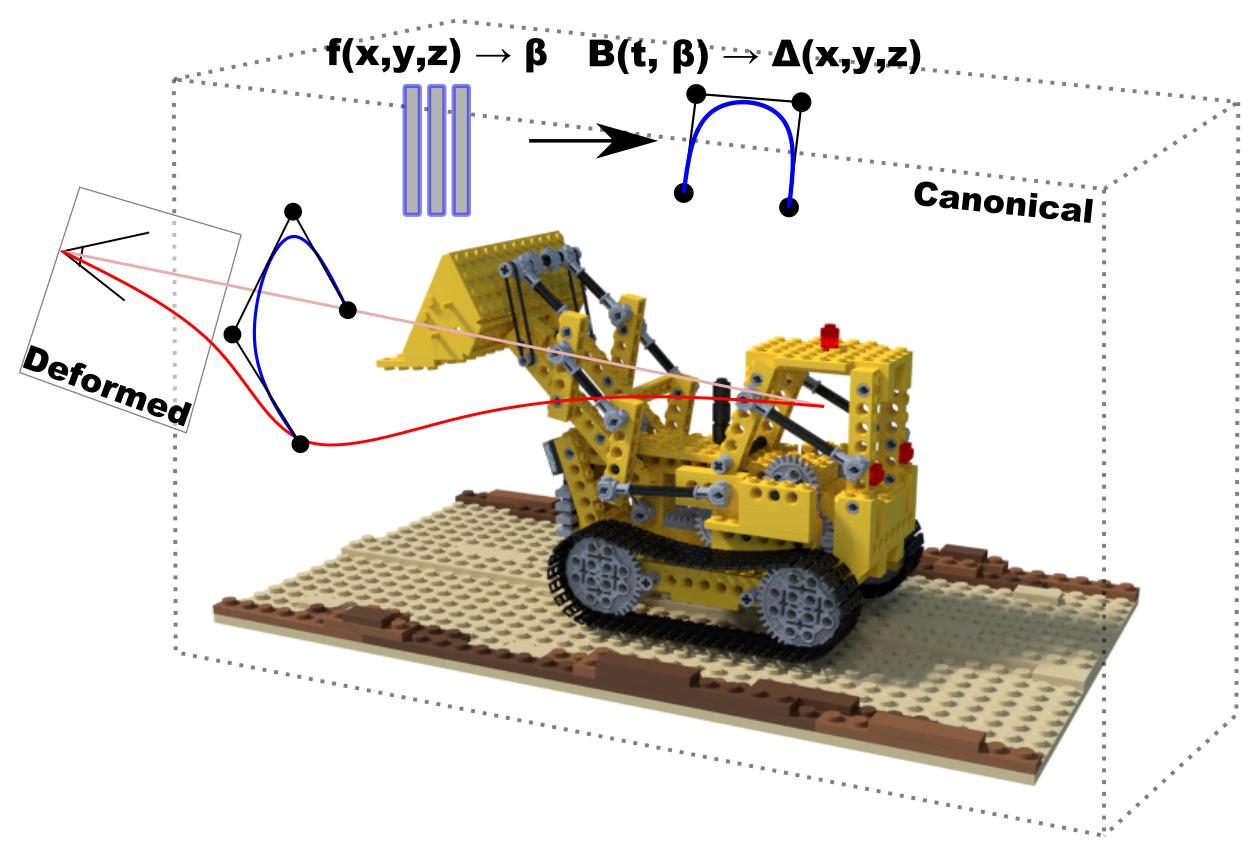
\includegraphics[width=\textwidth]{spline_nerf_diagram.png}
    \caption{
        \textbf{Spline-based Dynamic NeRF}. Instead of using an MLP to directly predict ray-bending ($\delta(x,y,z)$)  at a given time, we predict a set of Bezier spline control points. Then, we use the Bezier function to interpolate position based on time.
    }
    \label{fig:arch_diagram}
    \end{minipage}\hfill
    \begin{minipage}[b]{0.45\textwidth}
    \centering
    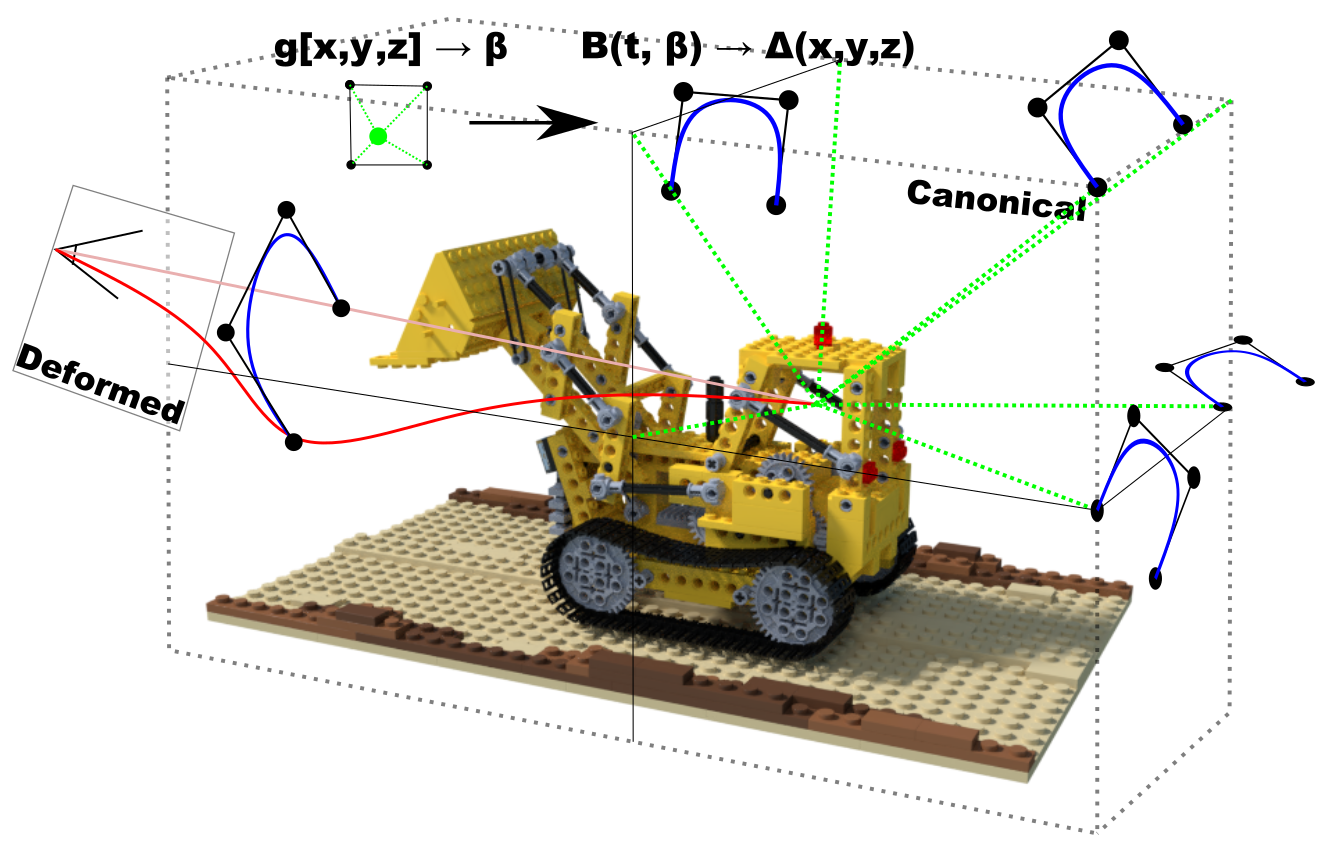
\includegraphics[width=\textwidth]{c0_paper/voxel_spline.png}
    \caption{
        \label{fig:voxel_diagram}
        \textbf{Voxelized spline-based Dynamic-NeRF}. At each voxel coordinate, we store an additional set of control points which are used for ray-bending. This allows us to efficiently and sparsely bend rays, without needing to query an MLP. Our implementation shares much of the same code as the MLP-based approach, but has better memory usage.
    }
    \end{minipage}
\end{figure*}